\documentclass[border=0pt]{standalone}
\usepackage{amsmath}
\usepackage[usenames,dvipsnames]{xcolor}
\usepackage{graphicx}

%%font
\usepackage{euler}
\usepackage[OT1]{eulervm}
\renewcommand{\rmdefault}{pplx}

\usepackage{amsmath, amssymb}
\usepackage{bigints}
\usepackage[hidelinks]{hyperref}

\newcommand{\bx}{\mathbf{x}}
\newcommand{\by}{\mathbf{y}}
\newcommand{\bu}{\mathbf{u}}
\newcommand{\bv}{\mathbf{v}}

\setcounter{MaxMatrixCols}{20}

\usepackage{tikz}
\tikzset{roundnode/.style={circle,draw=black,fill=blue!20}, 
every label/.style={rectangle, draw=none}}
\definecolor{TortugaColor}{rgb}{0.1,0.4,0.3}
\definecolor{Totemblue}{HTML}{09182F}
\definecolor{Totemred}{HTML}{2B030B}
\definecolor{Totemyellow}{HTML}{AD901B}
\usetikzlibrary{intersections}
%\usetikzlibrary{fadings}
\usetikzlibrary{arrows}
%\usetikzlibrary{arrows.meta}
%\usetikzlibrary{decorations}
\usetikzlibrary{decorations.pathmorphing}
\usetikzlibrary{decorations.text}
%% \usetikzlibrary{shadings}
%\usetikzlibrary{fit}
%\usetikzlibrary{calc}
%\usetikzlibrary{through}
%\usetikzlibrary{positioning}
%\usetikzlibrary{graphs}
%\usetikzlibrary{mindmap}
%\usetikzlibrary{backgrounds}
%\usetikzlibrary{calligraphy}
%% \usepgfmodule{nonlineartransformations}
%% \usetikzlibrary{curvilinear}

%%% Set up polar step (code from the pgd manual)
%\makeatletter
%\def\polartransformation{%
% \pgf@x will contain the radius
% \pgf@y will contain the distance
%\pgfmathsincos@{\pgf@sys@tonumber\pgf@x}%
% pgfmathresultx is now the cosine of radius and
% pgfmathresulty is the sine of radius
%\pgf@x=\pgfmathresultx\pgf@y%
%\pgf@y=\pgfmathresulty\pgf@y%
%}
%\makeatother

\pgfdeclarelayer{background}
\pgfdeclarelayer{alpha}
\pgfdeclarelayer{beta}
\pgfsetlayers{background,alpha,main,beta}

%%pic TaiJi
\tikzset{
TaiJi/.pic={
\begin{scope}[thick,yi/.style={radius=0.4cm}]
\shade [draw=black] (0,0) circle [radius =3];
\shade [top color=black, bottom color=black!50,draw=black] (0,-3) arc [radius=3, start angle=-90, end angle=90]
arc [radius=1.5, start angle=90, end angle=270]
arc [radius=1.5, start angle=90, end angle=-90];
\draw[thin,fill=black] (0,-1.5) circle [yi];
\draw[thin,fill=white] (0,1.5) circle [yi];
\end{scope}
}}

%%pic Totu
\tikzset{
totu/.pic={
\begin{scope}[scale=0.2]
\pgfmathsetmacro{\legwidth}{0.4*0.2}
\draw[fill=green!60!black!30] (0,0.8) circle [x radius=0.3,y radius=0.4];
\foreach \i in {-1,1}{
\begin{scope}[xscale=\i]
\path (0.8,0) edge[draw=green!60!black!30,line width=\legwidth cm,line cap=round,bend left] ++(0.6,0);
\path (0.6,-1) edge[draw=green!60!black!30,line width=\legwidth cm,line cap=round] ++ (0.4,-0.4);
\end{scope}
}
\draw (0,-1.4) edge[draw=green!60!black!30,line width=\legwidth cm,line cap=round] ++ (0,-0.4);
\draw[fill=green!60!black,rounded corners] (1,0) -- (0,0.5) -- (-1,0) -- (-0.8,-1.2) -- (0,-1.6) -- (0.8,-1.2) -- cycle;
\end{scope}
}}

%%pic Rescuer
\tikzset{
Rescuer/.pic={
\begin{scope}[shift={(6.35,1.2)}]
\draw[fill=black!20!red!60!yellow] (-7,-0.8) -- (-6.7,-1.2) -- (-6,-1.2) -- (-5.7,-0.8) .. controls +(-0.3,-0.1) and +(0.3,-0.1) ..  cycle;
\end{scope}
}}

%%pic SatanHeart
\tikzset{
SatanHeart/.pic={
\pgfmathsetmacro{\SatanHradius}{1}
\pgfmathsetmacro{\LSatanHradius}{1.05}
\begin{scope}[very thick]
\draw[gray!80!blue, line width=2pt] (0,0) circle[radius=\LSatanHradius cm];
\draw[gray!80!blue] (-90:\SatanHradius) -- (-306:\SatanHradius) -- (-162:\SatanHradius) -- (-378:\SatanHradius) -- (-234:\SatanHradius) -- cycle;
\end{scope}
}}

%%pic Stone Gate
\tikzset{
stonegate/.pic={
\begin{scope}[gray]
\draw[fill,draw=none,rounded corners] (-1.3,-0.3) rectangle (-0.7,2);
\draw[fill,draw=none,rounded corners] (0.7,-0.3) rectangle (1.3,2);
\draw[fill,draw=none] (0,2) ellipse[x radius=2cm, y radius=0.3cm];
\end{scope}
}}
 
%%pic Ateles Zombia
\tikzset{
zombia/.pic={
\pgfmathsetmacro{\zombiascale}{0.2}
\begin{scope}[scale=\zombiascale]
\pgfmathsetmacro{\zombiawidth}{\zombiascale *0.3 cm}
\pgfmathsetmacro{\zombiabigcorner}{\zombiascale *4 pt}
\pgfmathsetmacro{\zombiasmallcorner}{\zombiascale *0.2 cm}
\begin{scope}[gray!40, rounded corners=\zombiabigcorner, line width=\zombiawidth, line cap=round]
%\node[circle,draw,thin] at (0,0) {};
\draw [fill,thin] (-1.9,0.4) circle [radius=0.3cm];
\draw (-1.8,0.1) -- (-2.2,-0.3) -- (-2.7,-0.6);
\draw (-1.8,0.1) -- (-1.6,-0.8) -- ++ (0.1,-0.1);
\draw (-1.8,0.1) -- (-0.9,0.1) -- (0.4,0.8);
\draw[rounded corners=\zombiasmallcorner] (0.4,0.8) -- ++ (0.3,0.2) -- ++ (0.2,-0.2);
\draw (0.7,1) -- (0.9,1.3) -- (1,2.5) -- (1.3,3) -- (1.8,2.9);
\draw (0.9,0.8) -- (0.9,0.5) -- (0.95,-0.3) -- (0.8,-1.1);
\draw (0.8,0.8) -- (0.4,0.6) -- (0,-0.7) -- ++(-0.2,-0.2);
\end{scope}
\end{scope}
}
}

%%pic family
\tikzset{
family/.pic={
\begin{scope}[xshift=-1cm]
\clip (0,0) rectangle (2,1);
\draw[fill] (0.25,0.7) circle [radius=0.1cm];
\draw[line cap=round,line width=0.06cm] (0.25,0.7) -- (0.25,0.2);
\draw[line cap=round,line width=0.06cm] (0.15,0) -- (0.25,0.2) -- (0.35,0);

\draw[fill] (0.75,0.6) circle [radius=0.1cm];
\draw[line cap=round,line width=0.06cm] (0.75,0.6) -- (0.75,0.2);
\draw[line cap=round,line width=0.06cm] (0.65,0) -- (0.75,0.2) -- (0.85,0);

\draw[fill] (1.25,0.6) circle [radius=0.1cm];
\draw[line cap=round,line width=0.06cm] (1.25,0.6) -- (1.25,0.2);
\draw[line cap=round,line width=0.06cm] (1.15,0) -- (1.25,0.2) -- (1.35,0);

\draw[fill] (1.75,0.65) circle [radius=0.1cm];
\draw[line cap=round,line width=0.06cm] (1.75,0.65) -- (1.75,0.2);
\draw[line cap=round,line width=0.06cm] (1.65,0) -- (1.75,0.2) -- (1.85,0);

\draw[line cap=round, line width=0.06cm] (0,0.3) -- (0.25,0.5) -- (0.5,0.3) -- (0.75,0.4) -- (1,0.3) -- (1.25,0.4) -- (1.5,0.3) -- (1.75,0.45) -- (2,0.3);
\end{scope}
}
}

\parindent=0pt

\begin{document}
%%2024NewYear
%% 16:9
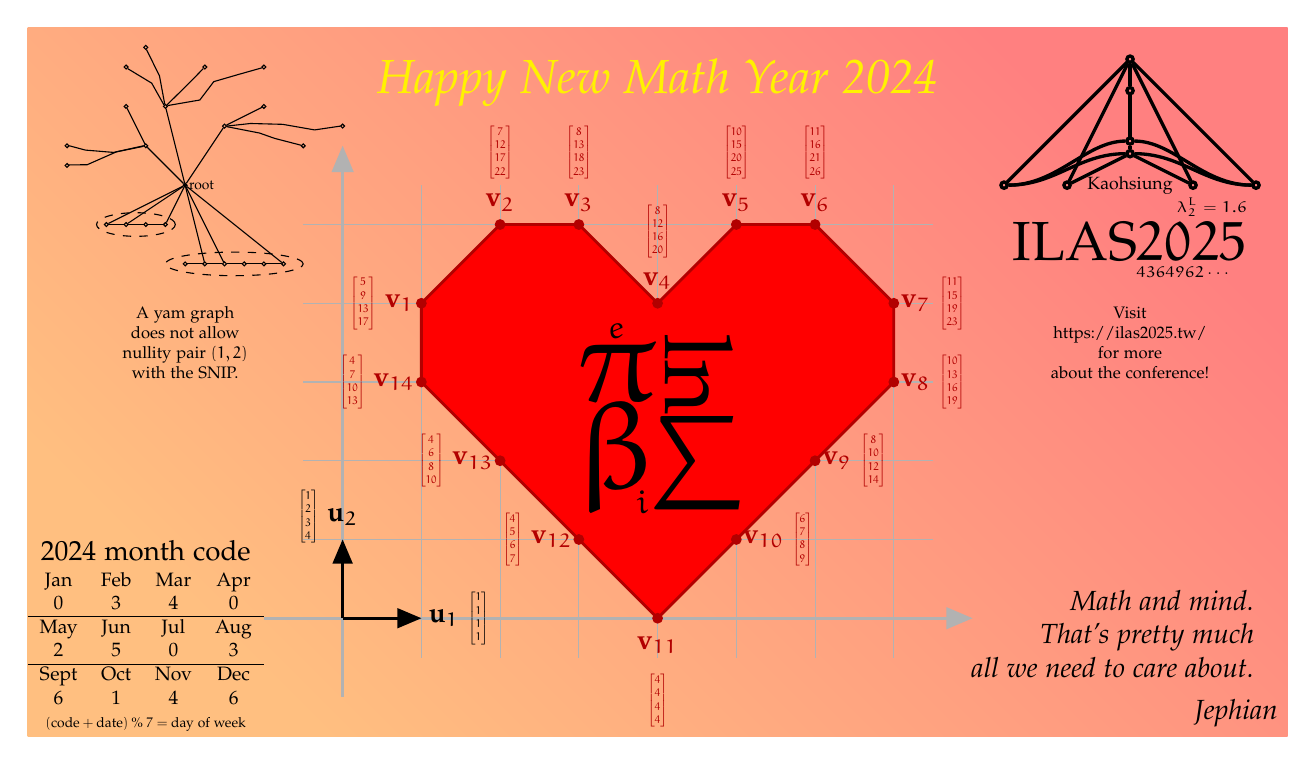
\begin{tikzpicture}
\coordinate (Jamaica) at (-8,-4);
\coordinate (Dominican) at (8,-4);
\coordinate (Cuba) at (-8,5);
\coordinate (TurksCaicos) at (8,5);
\coordinate (Tortuga) at (0,0);
\clip (Jamaica) rectangle (TurksCaicos);

%%Help Lines
\begin{pgfonlayer}{beta}
%% \draw [step=1, black!50, thin] (Jamaica) grid (TurksCaicos);
%% \draw (0,0) circle [radius=0.2cm];
\end{pgfonlayer}


%%background Layer
\begin{pgfonlayer}{background}
%% \shade [inner color=red!70, outer color=orange!50] (-8,-4) rectangle (8,5);
%% \shade [left color=orange, right color=red!70] (-8,-4) rectangle (8,5);
\shade [shading=axis, top color=orange!50, bottom color=red!50, shading angle=135] (-8,-4) rectangle (8,5);
%% \begin{scope}[opacity=0.2]
%% \foreach \i in {1,2,3,4} {
%%     \pgfmathsetmacro{\ang}{180 - 18 * \i}
%%     \pgfmathsetmacro{\rang}{180 + \ang}
%%     \pic[xshift=-0.5cm, rotate=\rang] at (\ang:3) {totu};
%% }
%% \foreach \i in {1,2,3,4} {
%%     \pgfmathsetmacro{\ang}{270 + 18 * \i}
%%     \pgfmathsetmacro{\rang}{\ang}
%%     \pic[xshift=0.5cm, rotate=\rang] at (\ang:3) {totu};
%% }
%% \end{scope
%% }
\end{pgfonlayer} 


%%Main Layer (main)
\begin{pgfonlayer}{main}

%%% HD HEART
\begin{scope}[xshift=-4cm, yshift=-2.5cm,every node/.style={draw, circle, inner sep=1pt}, line width=1pt]
\pgfmathsetmacro{\vscale}{0.4}
  
  %%% coordinates
  \begin{scope}[black!30]
    \draw[very thick, -triangle 45] (-1,0) -- (8,0);
    \draw[very thick, -triangle 45] (0,-1) -- (0,6);  
    \foreach \y in {1,2,...,5} {
      \draw[thin] (-0.5,\y) -- (7.5,\y);
    }
    \foreach \x in {1,2,...,7} {
      \draw[thin] (\x,-0.5) -- (\x,5.5);
    }
  \end{scope}

  %%% heart
  \begin{scope}[red!70!black]
    \fill[draw, fill=red] (1,4) coordinate (v1) --
    (2,5) coordinate (v2)  --
    (3,5) coordinate (v3) --
    (4,4) coordinate (v4) --
    (5,5) coordinate (v5) --
    (6,5) coordinate (v6) --
    (7,4) coordinate (v7) --
    (7,3) coordinate (v8) --
    (6,2) coordinate (v9) --
    (5,1) coordinate (v10) --
    (4,0) coordinate (v11) --
    (3,1) coordinate (v12) --
    (2,2) coordinate (v13) --
    (1,3) coordinate (v14) --
    cycle;

    \foreach \i in {1,2,...,14} {
      \node[fill] at (v\i) {};
    }

    \node[left, draw=none] (lv1) at (v1) {$\bv_1$};
    \node[above, draw=none] (lv2) at (v2) {$\bv_2$};
    \node[above, draw=none] (lv3) at (v3) {$\bv_3$};
    \node[above, draw=none] (lv4) at (v4) {$\bv_4$};
    \node[above, draw=none] (lv5) at (v5) {$\bv_5$};
    \node[above, draw=none] (lv6) at (v6) {$\bv_6$};
    \node[right, draw=none] (lv7) at (v7) {$\bv_7$};
    \node[right, draw=none] (lv8) at (v8) {$\bv_8$};
    \node[right, draw=none] (lv9) at (v9) {$\bv_9$};
    \node[right, draw=none] (lv10) at (v10) {$\bv_{10}$};
    \node[below, draw=none] (lv11) at (v11) {$\bv_{11}$};
    \node[left, draw=none] (lv12) at (v12) {$\bv_{12}$};
    \node[left, draw=none] (lv13) at (v13) {$\bv_{13}$};
    \node[left, draw=none] (lv14) at (v14) {$\bv_{14}$};

    \node[draw=none, rectangle, scale=\vscale, left] at (lv1.west) {$\begin{bmatrix} 5 \\ 9 \\ 13 \\ 17 \end{bmatrix}$};
    \node[draw=none, rectangle, scale=\vscale, above] at (lv2.north) {$\begin{bmatrix} 7 \\ 12 \\ 17 \\ 22 \end{bmatrix}$};
    \node[draw=none, rectangle, scale=\vscale, above] at (lv3.north) {$\begin{bmatrix} 8 \\ 13 \\ 18 \\ 23 \end{bmatrix}$};
    \node[draw=none, rectangle, scale=\vscale, above] at (lv4.north) {$\begin{bmatrix} 8 \\ 12 \\ 16 \\ 20 \end{bmatrix}$};
    \node[draw=none, rectangle, scale=\vscale, above] at (lv5.north) {$\begin{bmatrix} 10 \\ 15 \\ 20 \\ 25 \end{bmatrix}$};
    \node[draw=none, rectangle, scale=\vscale, above] at (lv6.north) {$\begin{bmatrix} 11 \\ 16 \\ 21 \\ 26 \end{bmatrix}$};
    \node[draw=none, rectangle, scale=\vscale, right] at (lv7.east) {$\begin{bmatrix} 11 \\ 15 \\ 19 \\ 23 \end{bmatrix}$};
    \node[draw=none, rectangle, scale=\vscale, right] at (lv8.east) {$\begin{bmatrix} 10 \\ 13 \\ 16 \\ 19 \end{bmatrix}$};
    \node[draw=none, rectangle, scale=\vscale, right] at (lv9.east) {$\begin{bmatrix} 8 \\ 10 \\ 12 \\ 14 \end{bmatrix}$};
    \node[draw=none, rectangle, scale=\vscale, right] at (lv10.east) {$\begin{bmatrix} 6 \\ 7 \\ 8 \\ 9 \end{bmatrix}$};
    \node[draw=none, rectangle, scale=\vscale, below] at (lv11.south) {$\begin{bmatrix} 4 \\ 4 \\ 4 \\ 4 \end{bmatrix}$};
    \node[draw=none, rectangle, scale=\vscale, left] at (lv12.west) {$\begin{bmatrix} 4 \\ 5 \\ 6 \\ 7 \end{bmatrix}$};
    \node[draw=none, rectangle, scale=\vscale, left] at (lv13.west) {$\begin{bmatrix} 4 \\ 6 \\ 8 \\ 10 \end{bmatrix}$};
    \node[draw=none, rectangle, scale=\vscale, left] at (lv14.west) {$\begin{bmatrix} 4 \\ 7 \\ 10 \\ 13 \end{bmatrix}$};
    
  \end{scope}

  %%% points
  \begin{scope}[black]
    \draw[-triangle 45] (0,0) -- (1,0) node[right, draw=none] (u1) {$\bu_1$};
    \draw[-triangle 45] (0,0) -- (0,1) node[above, draw=none] (u2) {$\bu_2$};

    \node[draw=none, rectangle, scale=\vscale, right] at (u1.east) {$\begin{bmatrix} 1 \\ 1 \\ 1 \\ 1 \end{bmatrix}$};
    \node[draw=none, rectangle, scale=\vscale, left] at (u2.west) {$\begin{bmatrix} 1 \\ 2 \\ 3 \\ 4 \end{bmatrix}$};
  \end{scope}
\end{scope}

%%% TABLE
%% \node[rectangle, scale=0.3] at (0,0) {
%%   \begin{tabular}{cc|cccccccccccccc}
%%     $\bu_1$ & $\bu_2$ & $\bv_1$ & $\bv_1$ & $\bv_1$ & $\bv_1$ & $\bv_1$ & $\bv_1$ & $\bv_1$ & $\bv_1$ & $\bv_1$ & $\bv_1$ & $\bv_1$ & $\bv_1$ & $\bv_1$ & $\bv_1$ \\
%%     \hline
%%     $\begin{bmatrix} 1 \\ 1 \\ 1 \\ 1 \end{bmatrix}$ & 
%%     $\begin{bmatrix} 1 \\ 2 \\ 3 \\ 4 \end{bmatrix}$ & 
%%     $\begin{bmatrix} 5 \\ 9 \\ 13 \\ 17 \end{bmatrix}$ & 
%%     $\begin{bmatrix} 7 \\ 12 \\ 17 \\ 22 \end{bmatrix}$ & 
%%     $\begin{bmatrix} 8 \\ 13 \\ 18 \\ 23 \end{bmatrix}$ & 
%%     $\begin{bmatrix} 8 \\ 12 \\ 16 \\ 20 \end{bmatrix}$ & 
%%     $\begin{bmatrix} 10 \\ 15 \\ 20 \\ 25 \end{bmatrix}$ & 
%%     $\begin{bmatrix} 11 \\ 16 \\ 21 \\ 26 \end{bmatrix}$ & 
%%     $\begin{bmatrix} 11 \\ 15 \\ 19 \\ 23 \end{bmatrix}$ & 
%%     $\begin{bmatrix} 10 \\ 13 \\ 16 \\ 19 \end{bmatrix}$ & 
%%     $\begin{bmatrix} 8 \\ 10 \\ 12 \\ 14 \end{bmatrix}$ & 
%%     $\begin{bmatrix} 6 \\ 7 \\ 8 \\ 9 \end{bmatrix}$ & 
%%     $\begin{bmatrix} 4 \\ 4 \\ 4 \\ 4 \end{bmatrix}$ & 
%%     $\begin{bmatrix} 4 \\ 5 \\ 6 \\ 7 \end{bmatrix}$ & 
%%     $\begin{bmatrix} 4 \\ 6 \\ 8 \\ 10 \end{bmatrix}$ & 
%%     $\begin{bmatrix} 4 \\ 7 \\ 10 \\ 13 \end{bmatrix}$
%%   \end{tabular}
%% };

%%% DRAGON
%% https://www.mdbg.net/chinese/dictionary?page=chardict&cdcanoce=0&cdqchi=%E9%BE%8D
\begin{scope}[scale=1.5, transform shape, draw=none, rectangle]
\node[scale=3] (dpi) at (-0.35,0.4) {$\pi$};
\node[yshift=-0.25cm, scale=0.75] (de) at (dpi.north) {$e$};

\node[scale=3] (dbeta) at (-0.35,-0.3) {$\beta$};
\node[xshift=-0.5cm, yshift=0.45cm, scale=0.8] (di) at (dbeta.south east) {$i$};

\node[scale=2.25, rotate=-90] (dln) at (0.35,0.4) {$\ln$};

\node[scale=2.25] (dsigma) at (0.35,-0.35) {$\sum$};
\end{scope}

%%% ILAS2025-LOGO
\begin{scope}[xshift=6cm, yshift=3cm, scale=0.8, transform shape, 
    every node/.style={circle, draw, inner sep=1pt}]
\begin{scope}[black, very thick]
\node (0) at (-2,0) {};
\node (1) at (-1,0) {};
\node (2) at (1,0) {};
\node (3) at (2,0) {};
\node (4) at (0,0.5) {};
\node (5) at (0,0.7) {};
\node (6) at (0,1.5) {};
\node (7) at (0,2) {};

\draw (7) -- (0);
\draw (7) -- (1);
\draw (7) -- (2);
\draw (7) -- (3);
\draw (4) -- (1);
\draw (4) -- (2);
\draw (4) -- (5) -- (6) -- (7);
\draw (4) to [out=180, in=0, out looseness=1] (0);
\draw (4) to [out=0, in=180, out looseness=1] (3);
\draw (5) to [out=180, in=0, out looseness=0.8] (0);
\draw (5) to [out=0, in=180, out looseness=0.8] (3);

\node[draw=none,rectangle] at (0,0) {\footnotesize Kaohsiung};
\end{scope}

% text
\begin{scope}[shift={(0,-0.9)}] % was -1.25
\node[rectangle, draw=none] (ILAS2025) at (0,0) {\Huge ILAS$2025$};
\node[rectangle, draw=none, above, xshift=1.3cm] at (ILAS2025.north) {\scriptsize$\lambda_2^L = 1.6$};
\node[rectangle, draw=none, below, xshift=0.86cm] at (ILAS2025.south) {\scriptsize$4364962\cdots$};
\end{scope}

\end{scope}

% URL
\node[draw=none, rectangle, align=center, scale=0.6, transform shape] at (6,1) {Visit\\\url{https://ilas2025.tw/}\\for more\\about the conference!};


%%% YAM
\begin{scope}[xshift=-6cm, yshift=3cm, scale=0.5, transform shape, 
  every node/.style={circle, draw, inner sep=1pt}]
\node[label={right:root}, fill] (root) at (0,0) {};

% leaf1
\node (l11) at (-1,1) {};
\node (l12) at (-1.5,2) {};
\node (l13) at (-3,1) {};
\node (l14) at (-3,0.5) {};
\draw (root) -- (l11);
\draw decorate[decoration={name=random steps}] {(l11) -- (l12)};
\draw decorate[decoration={name=random steps}] {(l11) -- (l13)};
\draw decorate[decoration={name=random steps}] {(l11) -- (l14)};

% leaf2
\node (l21) at (-0.5,2) {};
\node (l22) at (-1.5,3) {};
\node (l23) at (-1,3.5) {};
\node (l24) at (0.5,3) {};
\node (l25) at (2,3) {};
\draw (root) -- (l21);
\draw decorate[decoration={name=random steps}] {(l21) -- (l22)};
\draw decorate[decoration={name=random steps}] {(l21) -- (l23)};
\draw decorate[decoration={name=random steps}] {(l21) -- (l24)};
\draw decorate[decoration={name=random steps}] {(l21) -- (l25)};

% leaf3
\node (l31) at (1,1.5) {};
\node (l32) at (2,2) {};
\node (l33) at (4,1.5) {};
\node (l34) at (3,1) {};
\draw (root) -- (l31);
\draw decorate[decoration={name=random steps}] {(l31) -- (l32)};
\draw decorate[decoration={name=random steps}] {(l31) -- (l33)};
\draw decorate[decoration={name=random steps}] {(l31) -- (l34)};

% yam1
\foreach \i in {1,2,3,4} {
    \pgfmathsetmacro{\x}{-2 + 0.5*(\i - 1)}
    \node (y1\i) at (\x,-1) {};
}
\draw (y11) -- (y12) -- (y13) -- (y14);
\draw (root) -- (y11);
\draw (root) -- (y12);
\draw (root) -- (y14);
\draw[dashed] (-1.25,-1) ellipse (1cm and 0.3cm); 

% yam2
\foreach \i in {1,2,3,4,5,6} {
    \pgfmathsetmacro{\x}{0 + 0.5*(\i - 1)}
    \node (y2\i) at (\x,-2) {};
}
\draw (y21) -- (y22) -- (y23) -- (y24) -- (y25) -- (y26);
\draw (root) -- (y22);
\draw (root) -- (y23);
\draw (root) -- (y26);
\draw[dashed] (1.25,-2) ellipse (1.75cm and 0.3cm);   
\end{scope}

% text
\node[draw=none, rectangle, align=center, scale=0.6, transform shape] at (-6,1) {A yam graph\\ does not allow\\ nullity pair $(1,2)$\\ with the SNIP.};

\end{pgfonlayer}


%%beta layer
\begin{pgfonlayer}{beta}

%%Happy New Math Year
%\draw[decorate,decoration={text along path,text={|\color{red!80!yellow} \LARGE \it|Happy New Math Year 2020}}] (-3.5,-2.5) .. controls (-1,4.5) and (1,4.5) .. (3.5,-2.5);
%% \node[rectangle, draw=none, orange!80!yellow] at (0,-3) {\LARGE\it Happy New Math Year 2023};
\node[rectangle, draw=none, yellow] (hny) at (0,4.3) {\LARGE\it Happy New Math Year 2024};
%% \draw[yellow, very thick, -triangle 45, shorten <=0.1cm, shorten >=0.1cm] (hny.20) .. controls ++(0,2) and ++(0,-2) .. (2023.south);
%% \node[rectangle, draw=none, opacity=0] at (0,-0.5) {\Huge\tt FREE HONG KONG};

%%Month code
\node[above] at (-6.5,-1.9) {2024 month code};
\node[scale=0.7,below] at (-6.5,-1.8) {\begin{tabular}{cccc} 
Jan & Feb & Mar & Apr \\
 0 & 3 & 4 & 0 \\
\hline
May & Jun & Jul & Aug \\
 2 & 5 & 0 & 3 \\
\hline
Sept & Oct & Nov & Dec \\
 6 & 1 & 4 & 6 \\
\end{tabular}};
\node[scale=0.5,above] at (-6.5,-4) {$(\text{code}+\text{date})\mathbin{\%}7=\text{day of week}$};

%%Goal
% y 1.3 for three sentences
\node[yshift=1.3cm, xshift=-0.3cm, left, align=right] at (Dominican) {
\it Math and mind. \\
\it That's pretty much \\
\it all we need to care about.};

%%Signature
\node[yshift=0.3cm,left] at (Dominican) {\it Jephian};

\end{pgfonlayer}




\end{tikzpicture}
\end{document}


%%\draw=\path[draw]
%%\clip=\path[clip]
%%\graph=\path[graph]
%%bend right ~ bend right=30 ~ in,out=right30, left 30
%%(left:2)=(180:2)
%%left ~ anchor=east ~ anchor 0
%%for sharp corners: line cap, line joint
%%for elliptical rectangle: smooth circle, plot coordinates, tensions
%For updating 2.10 to 3.0.0
%after moving the folder, it requires 
%sudo texhash 
% to make it work.
%%To convert to jpg: compile the pdf first, and then use the command below
%% convert -density 300 file.pdf -quality 90 file.jpg
%% required to install imagemagick

%% use pdf2png in AUR with Resolution 500 for 2018 
%% use gimp for 2019 (resolution 1890 x 1062, export quality 90)

%% Sample transformation as below
\makeatletter
\def\mytrans{
    \pgfmathparse{\pgf@x+1cm}
    %\pgf@x=\pgfmathresult pt
    \pgfmathsetlength{\pgf@x}{\pgfmathresult pt}
}
\makeatother



